%\chapter{Python: k-means example, importing data, visualization, tic/toc}
\chapterauthor{Jonathan Baker}

\epigraph{Science without math is superstition.}{Jared Webb}

\minitoc

\section{Reading from files}
Here is an example of a program the reads the contents of a file:
\begin{tsession}{mycodebg}
\begin{verbatim}
# Use a list of lists to store comma-separated data from a file

rows = []
with open('my_data.csv','r') as reader:
    for line in reader:
        # Remove the newline character
        line = line.strip()
        # Make a list of the strings found between commas
        fields = line.splti(',')
        rows.append(fields)
\end{verbatim}
\end{tsession}
The \texttt{open} function can give you an iterable object that will read each line in a file.
The \texttt{'r'} tells Python that you want to read from the file.
The \texttt{with-as} commands create a special code block
that will automatically close the file reader for you,
even if your program crashes.

\section{Writing to files}
The \texttt{open} function can also open a file for writing.
Here is an example of a program the writes strings to a file:
\begin{tsession}{mycodebg}
\begin{verbatim}
# Write some strings to a file

title = "Ode to Spot"
lines = [ 'Felis Catus' , 'is your taxonomic nomenclature' ]

with open('my_poem.txt','w') as writer:
    writer.write(title)
    writer.write('\n')
    for line in lines:
        writer.write(line)
        writer.write('\n')
\end{verbatim}
\end{tsession}
The \texttt{'w'} argument tells \texttt{open}that you want to write to the file.
In \texttt{'w'} mode, the \texttt{open} function will erase
any existing contents of the file before writing begins.

You could instead use append mode by giving the parameter \texttt{'a'}.
The resulting writer object will put anything you write after the file's current contents.

\section{Numpy}
NumPy is the basic scientific computing package for Python.
It provides high-quality implementations of
\begin{itemize}
    \item N-dimensional array objects (think matrices and vectors).
    \item Common mathematical functions like sine.
    \item Random number generators.
\end{itemize}
Install NumPy with the bash command
\begin{tsession}{mytermbg}
\begin{verbatim}
sudo apt-get install python3-numpy
\end{verbatim}
\end{tsession}
\section{1-dimensional arrays}
The most important thing you get from NumPy is the Array type.
It behaves a little like a list, but it can be multi-dimensional
and supports basic arithmetic operations.
Some important differences between NumPy arrays and lists
appear in Table~\ref{tab0array}.
\begin{table}[htb!]
\centering
\begin{tabular}{l|l}
Python lists & NumPy Arrays\\
\hline
Entry-wise operations performed manually
& Entry-wise arithmetic automated\\
Multiple dimensions can be implemented manually 
& Fast multi-dimensional support and slicing\\
Can grow or shrink
& Fixed size (must reallocate memory to grow)\\
Can hold various types simultaneously & Hold only a single type\\
\end{tabular}
\caption{Feature comparison of NumPy arrays and built-in Python list}
\label{tab0array}
\end{table}
Below is an example demonstrating creation of a NumPy array
and how it behaves differently from a list.
\begin{tsession}{mypythonbg}
\begin{verbatim}
>>> import numpy as np

>>> b=[7,4,5]
>>> a=np.array(b)    ## Create an array from a list

>>> a                ## Display the array and the list
array([7, 4, 5])
>>> b
[7, 4, 5]

>>> a[0]             ## Access entries
7
>>> b[0]
7

>>> a.dtype          ## Check what type the array holds
dtype('int64')


>>> a*2              ## Compare scalar multiplication on array and list
array([14,  8, 10])
>>> b*2
[7, 4, 5, 7, 4, 5]

>>> a+3              ## Compare scalar addition on array and list
array([10,  7,  8])
>>> b+3
Traceback (most recent call last):
  File "<stdin>", line 1, in <module>
TypeError: can only concatenate list (not "int") to list

>>> a+[3]           ## Compare addition of a list on array and list
array([10,  7,  8])
>>> b+[3]
[7, 4, 5, 3]
>>> a+[3,4]
Traceback (most recent call last):
  File "<stdin>", line 1, in <module>
ValueError: operands could not be broadcast together with shapes (3,) (2,) 
>>> b+[3,4]
[7, 4, 5, 3, 4]
>>> a+[3,4,5]
array([10,  8, 10])
>>> b+[3,4,5]
[7, 4, 5, 3, 4, 5]

>>> c=a/4          ## Compare scalar addition on array and list
>>> c
array([1.75, 1.  , 1.25])
>>> c.dtype
dtype('float64')

>>> a.shape        ## shape of an array is a tuple
(3,)
>>> len(b)         ## len of a list is an int
3
\end{verbatim}
\end{tsession}
\section{Making higher-dimensional arrays}
2-dimensional arrays are also very common.
\begin{itemize}
    \item A 1-dimensional array represents a vector (similar to a list).
    \item A 2-dimensional array represents a matrix (similar to a list of lists.
    \item A higher dimensional array is similar to a list of lists of lists$\dots$.
\end{itemize}
Here are some common ways to create arrays with more than one dimension.
\begin{tsession}{mypythonbg}
\begin{verbatim}
>>> import numpy as np

>>> a=np.zeros( [3,4] )                ## Make a matrix with zeros/ones
>>> a                                  ## Notice that parameter is list
array([[0., 0., 0., 0.],
       [0., 0., 0., 0.],
       [0., 0., 0., 0.]])
>>> a.shape
(3, 4)
>>> a.dtype
dtype('float64')
>>> a.ndim
2

>>> a=np.ones([3,4])
>>> a
array([[1., 1., 1., 1.],
       [1., 1., 1., 1.],
       [1., 1., 1., 1.]])

>>> a=np.array(range(12)).reshape(3,4) ## Make a matrix with reshape
>>> a
array([[ 0,  1,  2,  3],
       [ 4,  5,  6,  7],
       [ 8,  9, 10, 11]])
>>> a.dtype
dtype('int64')
>>> a.shape
(3, 4)

>>> a=np.array(range(12))
>>> a.shape=(3,4)                      ## Assigning the shape directly is similar to reshape
>>> a
array([[ 0,  1,  2,  3],
       [ 4,  5,  6,  7],
       [ 8,  9, 10, 11]])

>>> a=np.array(range(20))
>>> a.shape=(4,-1)                      ## Shape of -1 automatically adapts to be the correct size
>>> a
array([[ 0,  1,  2,  3,  4],
       [ 5,  6,  7,  8,  9],
       [10, 11, 12, 13, 14],
       [15, 16, 17, 18, 19]])

>>> a=np.zeros([2,3,4,5])
>>> a
array([[[[0., 0., 0., 0., 0.],
         [0., 0., 0., 0., 0.],
         [0., 0., 0., 0., 0.],
         [0., 0., 0., 0., 0.]],

        [[0., 0., 0., 0., 0.],
         [0., 0., 0., 0., 0.],
         [0., 0., 0., 0., 0.],
         [0., 0., 0., 0., 0.]],

        [[0., 0., 0., 0., 0.],
         [0., 0., 0., 0., 0.],
         [0., 0., 0., 0., 0.],
         [0., 0., 0., 0., 0.]]],


       [[[0., 0., 0., 0., 0.],
         [0., 0., 0., 0., 0.],
         [0., 0., 0., 0., 0.],
         [0., 0., 0., 0., 0.]],

        [[0., 0., 0., 0., 0.],
         [0., 0., 0., 0., 0.],
         [0., 0., 0., 0., 0.],
         [0., 0., 0., 0., 0.]],

        [[0., 0., 0., 0., 0.],
         [0., 0., 0., 0., 0.],
         [0., 0., 0., 0., 0.],
         [0., 0., 0., 0., 0.]]]])
>>> a.shape
(2, 3, 4, 5)
>>> a.ndim

>>> np.set_printoptions(4)             ## Reduce displayed decimal places for readability
>>> np.empty([3,4])                    ## Allocate memory without initializing any value
array([[ -0.0000e+000,  -0.0000e+000,   2.1777e-314,   2.1777e-314],
       [  6.8878e-225,   0.0000e+000,   4.9003e+199,   3.2041e+204],
       [  1.7306e-077,  -0.0000e+000,   4.5458e+247,   2.9787e+252]])

>>> np.random.rand(3,4)                ## Random floats from 0 to 1 (parameters are ints, not list)
array([[ 0.13068673,  0.061761  ,  0.08081025,  0.89899938],
       [ 0.1787468 ,  0.63959114,  0.70993707,  0.50904187],
       [ 0.01586496,  0.43351682,  0.11899855,  0.64906669]])4
>>> np.random.randn(3,4)               ## Random normally distributed floats
array([[-0.37276598,  1.27200393,  1.35776972,  1.14684778],
       [-0.14485457,  1.68889778,  0.8922178 ,  1.61376074],
       [-0.11287411,  0.74026635, -1.1596352 ,  1.84264693]])
\end{verbatim}
\end{tsession}
\section{Reading and writing to arrays}
Entries of arrays can be accessed or assigned individually,
with slices (using \texttt{:}),
or with iterables (like lists).
The next interpreter example shows how these work.
\begin{tsession}{mypythonbg}
\begin{verbatim}
>>> import numpy as np

>>> a=np.array(range(12)).reshape(3,4)
>>> a
array([[ 0,  1,  2,  3],
       [ 4,  5,  6,  7],
       [ 8,  9, 10, 11]])
>>> a[1]                     ## A single index refers to a row
array([4, 5, 6, 7])
>>> a[1,2]                   ## Multiple indices are required to get a single entry
6

>>> a[:,1]                   ## Colon refers to all values in a dimension (result is 1-dimensional)
array([1, 5, 9])
>>> a[1,:]
array([4, 5, 6, 7])

>>> a[0:2,1:3]               ## Colon can also refer to a range of rows or columns
array([[1, 2],
       [5, 6]])

>>> a[2]=range(100,0,-25)    ## You can assign a whole row (or column) at a time
>>> a
array([[  0,   1,   2,   3],
       [  4,   5,   6,   7],
       [100,  75,  50,  25]])
>>> a[range(3),range(3)]=99 
>>> a[[0,1,0,0,2],[1,0,0,2,2]]=99
>>> a                        ## Assign scattered with lists of index pairs
array([[ 99,  99,  99,   3],
       [ 99,   5,   6,   7],
       [100,  75,  99,  25]])

>>> a[:,:]=6                 ## Assign all values at once
>>> a
array([[6, 6, 6, 6],
       [6, 6, 6, 6],
       [6, 6, 6, 6]])
\end{verbatim}
\end{tsession}

\section{Slicing and memory}
NumPy arrays are designed for fast arithmetic.
Consequently, the data in NumPy arrays must be stored in very particular ways.
When you make a new array out of a portion of an existing array,
NumPy would like to avoid copying the data,
but it can only avoid copying if you ask for data that appears in a certain pattern
\underline{and} you use ``slicing'' notation.
When you slice an array, NumPy does not copy data;
it just gives you a reference or ``view'' of the original data.

Slicing is achieved with special indexing notation using colons (\texttt{:}).
Slicing notation is similar to the parameters of the \texttt{range} function.
The expression \texttt{a:b:c} means ``start at entry \texttt{a} and take every \texttt{c}th entry until \texttt{b} is reached.''
Element \texttt{b} is not included in the slice.
The letters each has a default value (\texttt{a}=0, \texttt{b}=length+1, \texttt{c}=1),
so any of them can be omitted.

Below are some examples of the results of slicing a 1-dimensional array.
\begin{tsession}{mypythonbg}
\begin{verbatim}
>>> import numpy as np

>>> a=np.array(range(12))
>>> a
array([ 0,  1,  2,  3,  4,  5,  6,  7,  8,  9, 10, 11])

>>> a[1:8:2]
array([1, 3, 5, 7])

>>> a[1:8]
array([1, 2, 3, 4, 5, 6, 7])

>>> a[:8]
array([0, 1, 2, 3, 4, 5, 6, 7])

>>> a[:8:4]
array([0, 4])

>>> a[:8:5]
array([0, 5])

>>> a[1::5]
array([ 1,  6, 11])

>>> a[1:]
array([ 1,  2,  3,  4,  5,  6,  7,  8,  9, 10, 11])

>>> a[::-1]                         ## Reversing entries is easy
array([11, 10,  9,  8,  7,  6,  5,  4,  3,  2,  1,  0])
\end{verbatim}
\end{tsession}
Multi-dimensional arrays can be sliced separately in each dimension.
You can also slice one dimension but use a different type of index on another dimension.
The result of the slice-and-non-slice operation is a copied array, not a view.

When the data is sliced instead of copied,
changes to the view change the original.
\begin{tsession}{mypythonbg}
\begin{verbatim}
>>> import numpy as np

>>> a=np.random.randint(0,100,7)   ## 7 random integers from 0 to 99
>>> a
array([14, 85, 39, 96, 89, 34, 32])

>>> b=a[0]                          ## Individual elements are returned by value
>>> b
14
>>> b=77
>>> a
array([14, 85, 39, 96, 89, 34, 32])

>>> c=a[2:4]                        ## Slices are returned by reference
>>> c
array([39, 96])
>>> c[0]=10000                      ## Changing a value in a slice changes the original
>>> c
array([10000,    96])
>>> a
array([   14,    85, 10000,    96,    89,    34,    32])

>>> d=a[[2,3]]                      ## Other indexing types produce copies
>>> d
array([10000,    96])
>>> d[0]=0                          ## Changing the copy does not change the original
>>> d
array([ 0, 96])
>>> a
array([   14,    85, 10000,    96,    89,    34,    32])

>>> a=np.array(range(12)).reshape([3,4])
>>> a
array([[ 0,  1,  2,  3],
       [ 4,  5,  6,  7],
       [ 8,  9, 10, 11]])
>>> b=a[[0,2],1:3]                  ## If any dimension is not sliced, data is copied
>>> b
array([[ 1,  2],
       [ 9, 10]])
>>> b[:,:]=0                        ## Changing the copy does not change the original
>>> b
array([[0, 0],
       [0, 0]])
>>> a
array([[ 0,  1,  2,  3],
       [ 4,  5,  6,  7],
       [ 8,  9, 10, 11]])
\end{verbatim}
\end{tsession}

\section{Other array operations}
NumPy provides several functions for convenience when working with arrays.
\begin{tsession}{mypythonbg}
\begin{verbatim}
>>> import numpy as np

>>> a=np.array(range(12)).reshape([3,4])
>>> a
array([[ 0,  1,  2,  3],
       [ 4,  5,  6,  7],
       [ 8,  9, 10, 11]])

>>> b=a.T                   ## .T provides a VIEW of the transpose
>>> b
array([[ 0,  4,  8],
       [ 1,  5,  9],
       [ 2,  6, 10],
       [ 3,  7, 11]])
>>> b[0,0]=99
>>> a
array([[99,  1,  2,  3],
       [ 4,  5,  6,  7],
       [ 8,  9, 10, 11]])

>>> np.mean(a)              ## Mean of all values
5.5
>>> np.mean(a,0)            ## Column-wise mean
array([ 4.,  5.,  6.,  7.])
>>> np.mean(a,1)            ## Row-wise mean
array([ 1.5,  5.5,  9.5])

>>> np.max(a)               ## Maximum of all values
11
>>> np.min(a,0)             ## Column-wise minimum
array([0, 1, 2, 3])
>>> np.max(a,1)             ## Row-wise maximum
array([ 3,  7, 11])

>>> np.maximum(a,5)         ## The values of a or 5, whichever is greater
array([[ 5,  5,  5,  5],
       [ 5,  5,  6,  7],
       [ 8,  9, 10, 11]])

>>> a-7
array([[-7, -6, -5, -4],
       [-3, -2, -1,  0],
       [ 1,  2,  3,  4]])
>>> np.abs(a-7)             ## Scalar NumPy functions should all work entry-wise on arrays
array([[7, 6, 5, 4],
       [3, 2, 1, 0],
       [1, 2, 3, 4]])
>>> np.sin(a)
array([[ 0.    ,  0.8415,  0.9093,  0.1411],
       [-0.7568, -0.9589, -0.2794,  0.657 ],
       [ 0.9894,  0.4121, -0.544 , -1.    ]])
\end{verbatim}
\end{tsession}

\section{Linear algebra with NumPy}
Matrix multiplication is performed with the ``at'' sign (\texttt{@}).
The \texttt{linalg} module provides useful functions like \texttt{norm} and \texttt{eig}.
\begin{tsession}{mypythonbg}
\begin{verbatim}
>>> import numpy as np

>>> a=np.array(range(12)).reshape([3,4])
>>> b=np.array(range(4))
>>> a
array([[ 0,  1,  2,  3],
       [ 4,  5,  6,  7],
       [ 8,  9, 10, 11]])
>>> b
array([0, 1, 2, 3])
>>> a@b
array([14, 38, 62])

>>> np.linalg.norm(a)           ## By default, norm of matrix is spectral norm
22.494443758403985
>>> np.linalg.norm(b)           ## By default, norm of vector is 2-norm
3.7416573867739413

>>> a=np.array(range(4))        ## To do an outer product, vectors must be 2-dimensional
>>> b=np.array(range(5))
>>> a.shape=1,-1
>>> b.shape=-1,1
>>> a
array([[0, 1, 2, 3]])
>>> b
array([[0],
       [1],
       [2],
       [3],
       [4]])
>>> b@a
array([[ 0,  0,  0,  0],
       [ 0,  1,  2,  3],
       [ 0,  2,  4,  6],
       [ 0,  3,  6,  9],
       [ 0,  4,  8, 12]])

>>> X=np.array(range(16)).reshape(4,4)
>>> X
array([[ 0,  1,  2,  3],
       [ 4,  5,  6,  7],
       [ 8,  9, 10, 11],
       [12, 13, 14, 15]])
>>> E,V=np.linalg.eig(X)        ## Get eigenvalues and eigenvectors of a square matrix
>>> E
array([  3.2464e+01,  -2.4642e+00,  -1.9079e-15,   5.9410e-16])
>>> V
array([[-0.1142,  0.7328,  0.5404, -0.0267],
       [-0.33  ,  0.2897, -0.6541, -0.3722],
       [-0.5458, -0.1533, -0.313 ,  0.8244],
       [-0.7617, -0.5963,  0.4267, -0.4256]])
\end{verbatim}
\end{tsession}

\section{Matplotlib}
Matplotlib is a Python package that supports graphical plotting.
Its basic plotting commands are similar to those in MatLab.

The previous chapter used Matplotlib as an example of an external package that can be be installed with \texttt{apt-get}.
If you haven't already, install Matplotlib for Python 3 by typing at the bash terminal
\begin{tsession}{mytermbg}
\begin{verbatim}
sudo apt-get install python3-matplotlib
\end{verbatim}
\end{tsession}
Matplotlib has many features, but the simple \texttt{plot} function
will cover many of your needs.
The example below shows how to import the PyPlot package from Matplotlib,
plot points from data,
add labels and a legend,
save the plot as a file,
and display the plot in an interactive viewer.
\begin{tsession}{mycodebg}
\begin{verbatim}
# Draw a pair of sine waves with different colors and symbols

import matplotlib.pyplot as plt
import numpy as np

# 50 floats from 0 to 2*pi
x = np.linspace(0,2*np.pi,50)

y1 = np.sin(x)
y2 = np.cos(x)

# Plot the first curve in blue x's
plt.plot(x,y1,'bx')

# Plot the second curve with circles of a custom color
# and no line appearing between dots
plt.plot( x , y2 , marker='o' , color=[0.79, 0.17, 0.57] )

# Label the axes
plt.xlabel('x axis')
plt.ylabel('y axis')
plt.label('A pair of waves')

# Add a legend to explain the plot
plt.legend(['sin(x)','cos(x)'])

# Save the plot to an image file
plt.savefig('sines.png')

# Pause the program and display the plot in a GUI
plt.show()
\end{verbatim}
\end{tsession}
The resulting image from this program is shown in Figure~\ref{fig0sines}.
\begin{figure}[htb!]
    \centering
    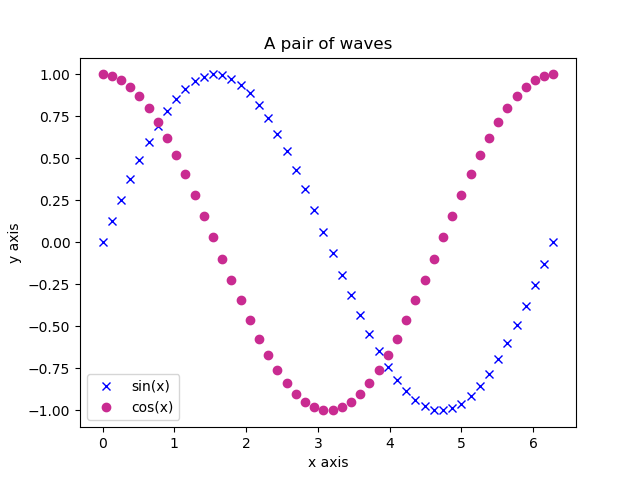
\includegraphics[width=0.9\textwidth]{figures/L12/sines.png}
    \caption{A plot by Matplotlib.}
    \label{fig0sines}
\end{figure}

% \section{Speed of Python vs C}
% So the students are aware:
% Show a Python implementation of Kmeans
% Show how speed compares to C
% Show some Cython

% In homework, students will:
% Export clusters from C
% Import clusters to python
% Visualize

\section{More information}

\begin{itemize}
    \item \href{https://numpy.org/devdocs/user/quickstart.html}{Numpy array tutorial}. Lots of details on how NumPy arrays work.
    \item \href{https://matplotlib.org/api/pyplot_api.html#matplotlib.pyplot.plot}{Matplotlib line specifications}.
    \item \href{https://matplotlib.org/3.1.1/gallery/index.html}{Matplotlib gallery}. If you want to make a special figure, you can probably find a related example here.
\end{itemize}


